\documentclass{article}

\usepackage[spanish]{babel}
\usepackage[numbers,sort&compress]{natbib}
\usepackage{graphicx}

\title{Reporte 1: Tarea de cosa tal}
\author{Jos\'{e} Antonio Pe\~{n}a P\'{e}rez}

\begin{document}

\maketitle

\section{Introducci\'{o}n}\label{intro}

Rollo con alguna cosa sin significado \citep{libro}.
Adem\'{a}s \citet{art} dice cosas importantes y se ven unos resultados
en la figura \ref{fig} y adem\'{a}s viene rollo en el cuadro \ref{datos}.

\begin{figure}
  \centering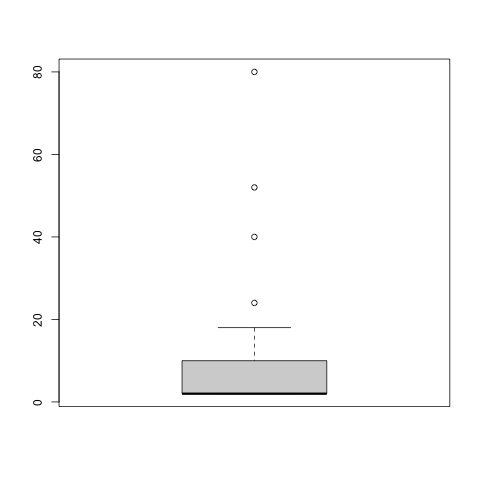
\includegraphics[width=0.5\textwidth]{demo.png}
  \caption{Un mal ejemplo porque no vienen etiquetas en los ejes.}
  \label{fig}
\end{figure}

\begin{table}
  \caption{Otro mal ejemplo pero ahora con datos.}
  \label{datos}
  \begin{center}
    \begin{tabular}{lr}
      M\'{\i}nimo & 2.00 \\
      M\'{a}ximo & 80.00 \\
      Promedio & 14.33
    \end{tabular}
  \end{center}
\end{table}


\section{Conclusiones}

En la secci\'{o}n \ref{intro}, hubo puro rollo.

\bibliography{ejemplo}
\bibliographystyle{plainnat}

\end{document}
